\chapter{Chapter 1}\label{ch:chapter01}

This is a template you can use for your thesis.
In the following some examples will be given how to use the template features.

\section{Some Section}\label{sec:some-section}
This is a section with some text.

\section{Lists}\label{sec:lists}
This is a list:
\begin{itemize}
    \item First item
    \item Second item
    \item Third item
\end{itemize}

\pagebreak

\section{Images}\label{sec:images}

\subsection{Simple Image}\label{subsec:simple-image}

This is an image:
\begin{figure}[h]
    \centering
    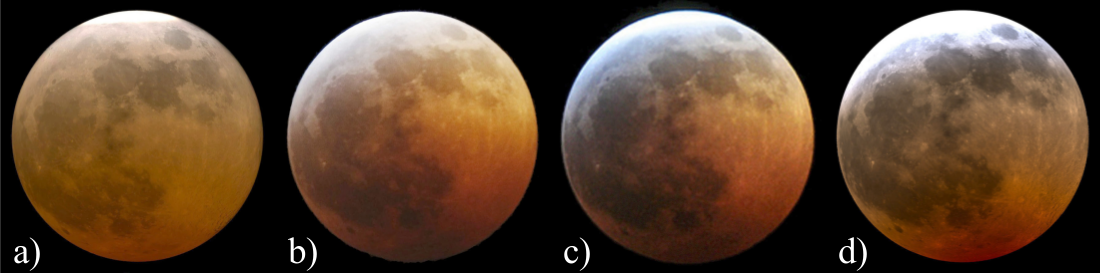
\includegraphics[width=\textwidth]{chapter01/images/Comparison_Yapo_Limberger}
    \caption{This is the image caption. The image is from Limberger et al.~\cite{Limberger2012}.}
    \label{fig:image-example}
\end{figure}


\subsection{Image Comparison}\label{subsec:image-comparison}
\begin{figure}[h]
    \begin{subfigure}[h]{0.45\textwidth}
        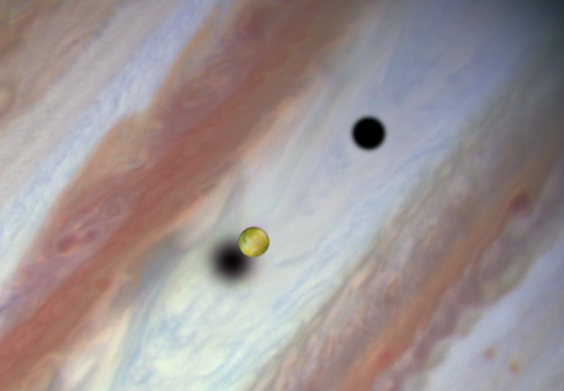
\includegraphics[width=\textwidth]{chapter01/images/HubbleJupiterEclipse2015}
    \end{subfigure}
    \hfill\vrule\hfill
    \begin{subfigure}[h]{0.45\textwidth}
        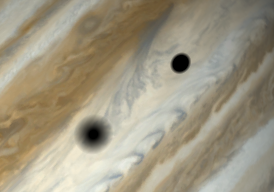
\includegraphics[width=\textwidth]{chapter01/images/CosmoGraphiaEclipseJupiter2015}
    \end{subfigure}

    \caption{Here you can see two images next to another for comparison.}
    \label{fig:image-comparison}
\end{figure}

\section{Citations and References}\label{sec:citations-and-references}
This is a citation: Limberger et al.~\cite{Limberger2012}.

This is a reference to the Appendix~\ref{ch:appendix}.

This is a reference to an image~\ref{fig:image-example}.

Here are some more citations for example purposes at the end of the paper:
\begin{itemize}
    \item Inproceedings~\cite{Yapo2009}
    \item Article~\cite{williams1978}
    \item Website~\cite{celestiaWebsite}
    \item Tech Report~\cite{usStandardAtmosphere}
    \item Master Thesis~\cite{fischer2018}
    \item Book~\cite{bohren1998}
\end{itemize}